% Capítulo 6: a pilha de chamadas durante media(n1, n2).
\documentclass[border=4pt]{standalone}
\usepackage[utf8]{inputenc}
\usepackage[T1]{fontenc}
% Estilo comum dos fluxogramas e diagramas de blocos.
\usepackage{tikz}
\usetikzlibrary{arrows.meta, positioning, calc, shapes.geometric, shapes.misc}
\definecolor{navy}{RGB}{23,45,80}
\definecolor{laranja}{RGB}{250,110,29}
\definecolor{cinzalogo}{RGB}{107,114,126}
\definecolor{azul}{RGB}{205,222,247}
\tikzset{
  base/.style={draw=navy, line width=0.9pt, font=\sffamily\small, align=center, inner sep=4pt},
  terminal/.style={base, rounded rectangle, fill=laranja!45, draw=laranja, minimum width=20mm, minimum height=7mm},
  processo/.style={base, rectangle, fill=laranja!12, minimum width=28mm, minimum height=8mm},
  decisao/.style={base, diamond, aspect=2.2, fill=azul, inner sep=1pt, minimum width=30mm},
  es/.style={base, trapezium, trapezium left angle=72, trapezium right angle=108,
             fill=white, minimum width=26mm, minimum height=8mm, trapezium stretches body},
  fluxo/.style={-{Stealth[length=2.2mm]}, navy, line width=0.9pt},
  rotulo/.style={font=\sffamily\small\bfseries, text=navy},
  legenda/.style={font=\sffamily\scriptsize, text=cinzalogo},
  resposta/.style={font=\sffamily\scriptsize\bfseries, text=navy},
}

\tikzset{
  registro/.style={draw=navy, line width=0.9pt, minimum width=44mm, minimum height=14mm, rounded corners=2pt},
  cx/.style={draw=navy, line width=0.7pt, minimum width=10mm, minimum height=6mm, font=\sffamily\small\bfseries, text=navy, fill=white},
  nomevar/.style={font=\ttfamily\scriptsize, text=navy},
  titulo/.style={font=\sffamily\small\bfseries, text=navy, anchor=north west},
  copia/.style={-{Stealth[length=2mm]}, laranja, line width=0.9pt},
}
\newcommand{\caixa}[4]{% x, y, nome, valor
  \node[cx] (#3) at (#1, #2) {#4};
  \node[nomevar] at (#1, #2+0.48) {#3};
}
\begin{document}
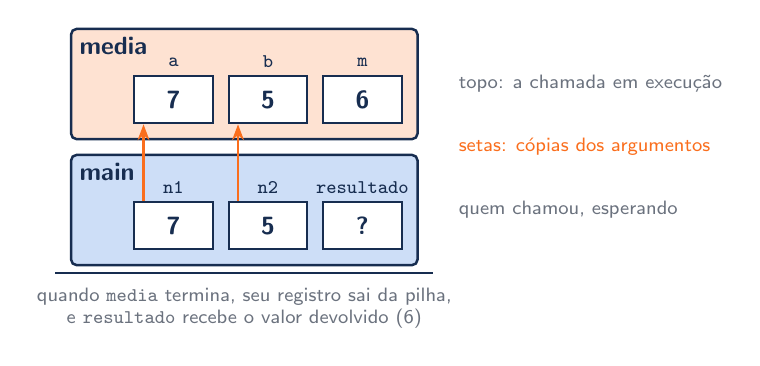
\begin{tikzpicture}
  % registro de media (topo)
  \node[registro, fill=laranja!20] (rm) at (0, 1.6) {};
  \node[titulo] at (rm.north west) {media};
  \caixa{-0.9}{1.4}{a}{7}
  \caixa{0.3}{1.4}{b}{5}
  \caixa{1.5}{1.4}{m}{6}
  % registro de main (base)
  \node[registro, fill=azul] (rmain) at (0, 0) {};
  \node[titulo] at (rmain.north west) {main};
  \caixa{-0.9}{-0.2}{n1}{7}
  \caixa{0.3}{-0.2}{n2}{5}
  \caixa{1.5}{-0.2}{resultado}{?}

  \draw[copia] ($(n1.north)+(-0.38, 0)$) -- ($(a.south)+(-0.38, 0)$);
  \draw[copia] ($(n2.north)+(-0.38, 0)$) -- ($(b.south)+(-0.38, 0)$);

  \draw[navy, line width=0.6pt] (-2.4, -0.8) -- (2.4, -0.8);
  \node[legenda, anchor=west] at (2.6, 1.6) {topo: a chamada em execução};
  \node[legenda, anchor=west] at (2.6, 0) {quem chamou, esperando};
  \node[legenda, anchor=west, text=laranja] at (2.6, 0.8) {setas: cópias dos argumentos};
  \node[legenda, align=center] at (0, -1.25) {quando \texttt{media} termina, seu registro sai da pilha,\\e \texttt{resultado} recebe o valor devolvido (6)};
\end{tikzpicture}
\end{document}
